\section{Basic Example Implementations}
In this chapter we'll show some example applications and implementations. These are in a minified version and do not necessarily represent the best practices that should be applied. Where ever possible, sources will be provided where those best practices can be read on.

\textit{These examples show versions where the sender and receiver are the same client. For a real world application those code parts would be separated. The needed communication information, like offer, answer or \index{ICE}{ICE} candidate, would be transferred through a signaling service which is not part of the \index{WebRTC}{WebRTC} specs. Additionally the \index{ICE}{ICE} candidates need to be negotiated between the peers. This will be explored in a following section.}

\subsection{Connect Client}
This examples shows in a minimal way, how to create a \index{WebRTC}{WebRTC} connection. Important in this case is, that the sender creates an offer which is then used to create the \lstinline[basicstyle=\ttfamily\color{black}]|localDescription| for the sender and the \lstinline[basicstyle=\ttfamily\color{black}]|remoteDescription| for the receiver. The receiver on the other hand creates an answer which is used to set the \lstinline[basicstyle=\ttfamily\color{black}]|localDescription| of the receiver and the \lstinline[basicstyle=\ttfamily\color{black}]|remoteDescription| of the sender.

\textit{Since sender and receiver are the same client we can set the \index{ICE}{ICE} candidate in a minimal way. These process would be more complex in a real world application.}
\lstinputlisting[label=Connect to a client,caption=Connect to a client,language=JavaScript, style=JavaScript]{examples/miniConnect.js}

\subsection{Disconnect Client}
The connection can be closed by simply call the close function of the \index{WebRTC}{WebRTC} connection.
\lstinputlisting[label=Disconnect from a client,caption=Disconnect from a client,language=JavaScript, style=JavaScript]{examples/disconnect.js}

\subsection{Sending Data}
In this section we will showcase the ability to transfer arbitrary data between peers. In our case we will send text data, but it could be data in any format.

\lstinputlisting[label=Sending data,caption=Sending data,language=JavaScript, style=JavaScript]{examples/sendData.js}

\subsection{Video Chat}

\subsubsection{Client Media Check}
We need to check if the current environment supports the needed \index{API}{API}'s. Here is an example of such a check.
\lstinputlisting[label=Check client media,caption=Check client media,language=JavaScript, style=JavaScript]{examples/featureCheck.js}

\subsubsection{Accessing Client Media}
In this example we see how client media, in this case video and audio, can be accessed. This action needs the users permission, which will be asked for by the browser automatically. In a real world example the application would need to handle the access denied case.

\lstinputlisting[label=Access client media,caption=Access client media,language=JavaScript, style=JavaScript]{examples/accessMedia.js}

\subsubsection{Send Media}
In the following example we will take a look on how media can be send between peers.

\lstinputlisting[label=Send media,caption=Send media,language=JavaScript, style=JavaScript]{examples/sendMedia.js}

\subsection{ICE Candidates}
In a real world application we need to gather possible \index{ICE}{ICE} candidates for our connection. This is achieved by gathering the sending clients \index{ICE}{ICE} candidates and exchange them with the \index{ICE}{ICE} candidates from the receiving client. This starts with the highest priority candidates and continues to the lowest until a common candidate is found. The \lstinline[basicstyle=\ttfamily\color{black}]|onicecandidate| event handler is used to listen for incoming \index{ICE}{ICE} candidates.

\begin{figure}[H]
	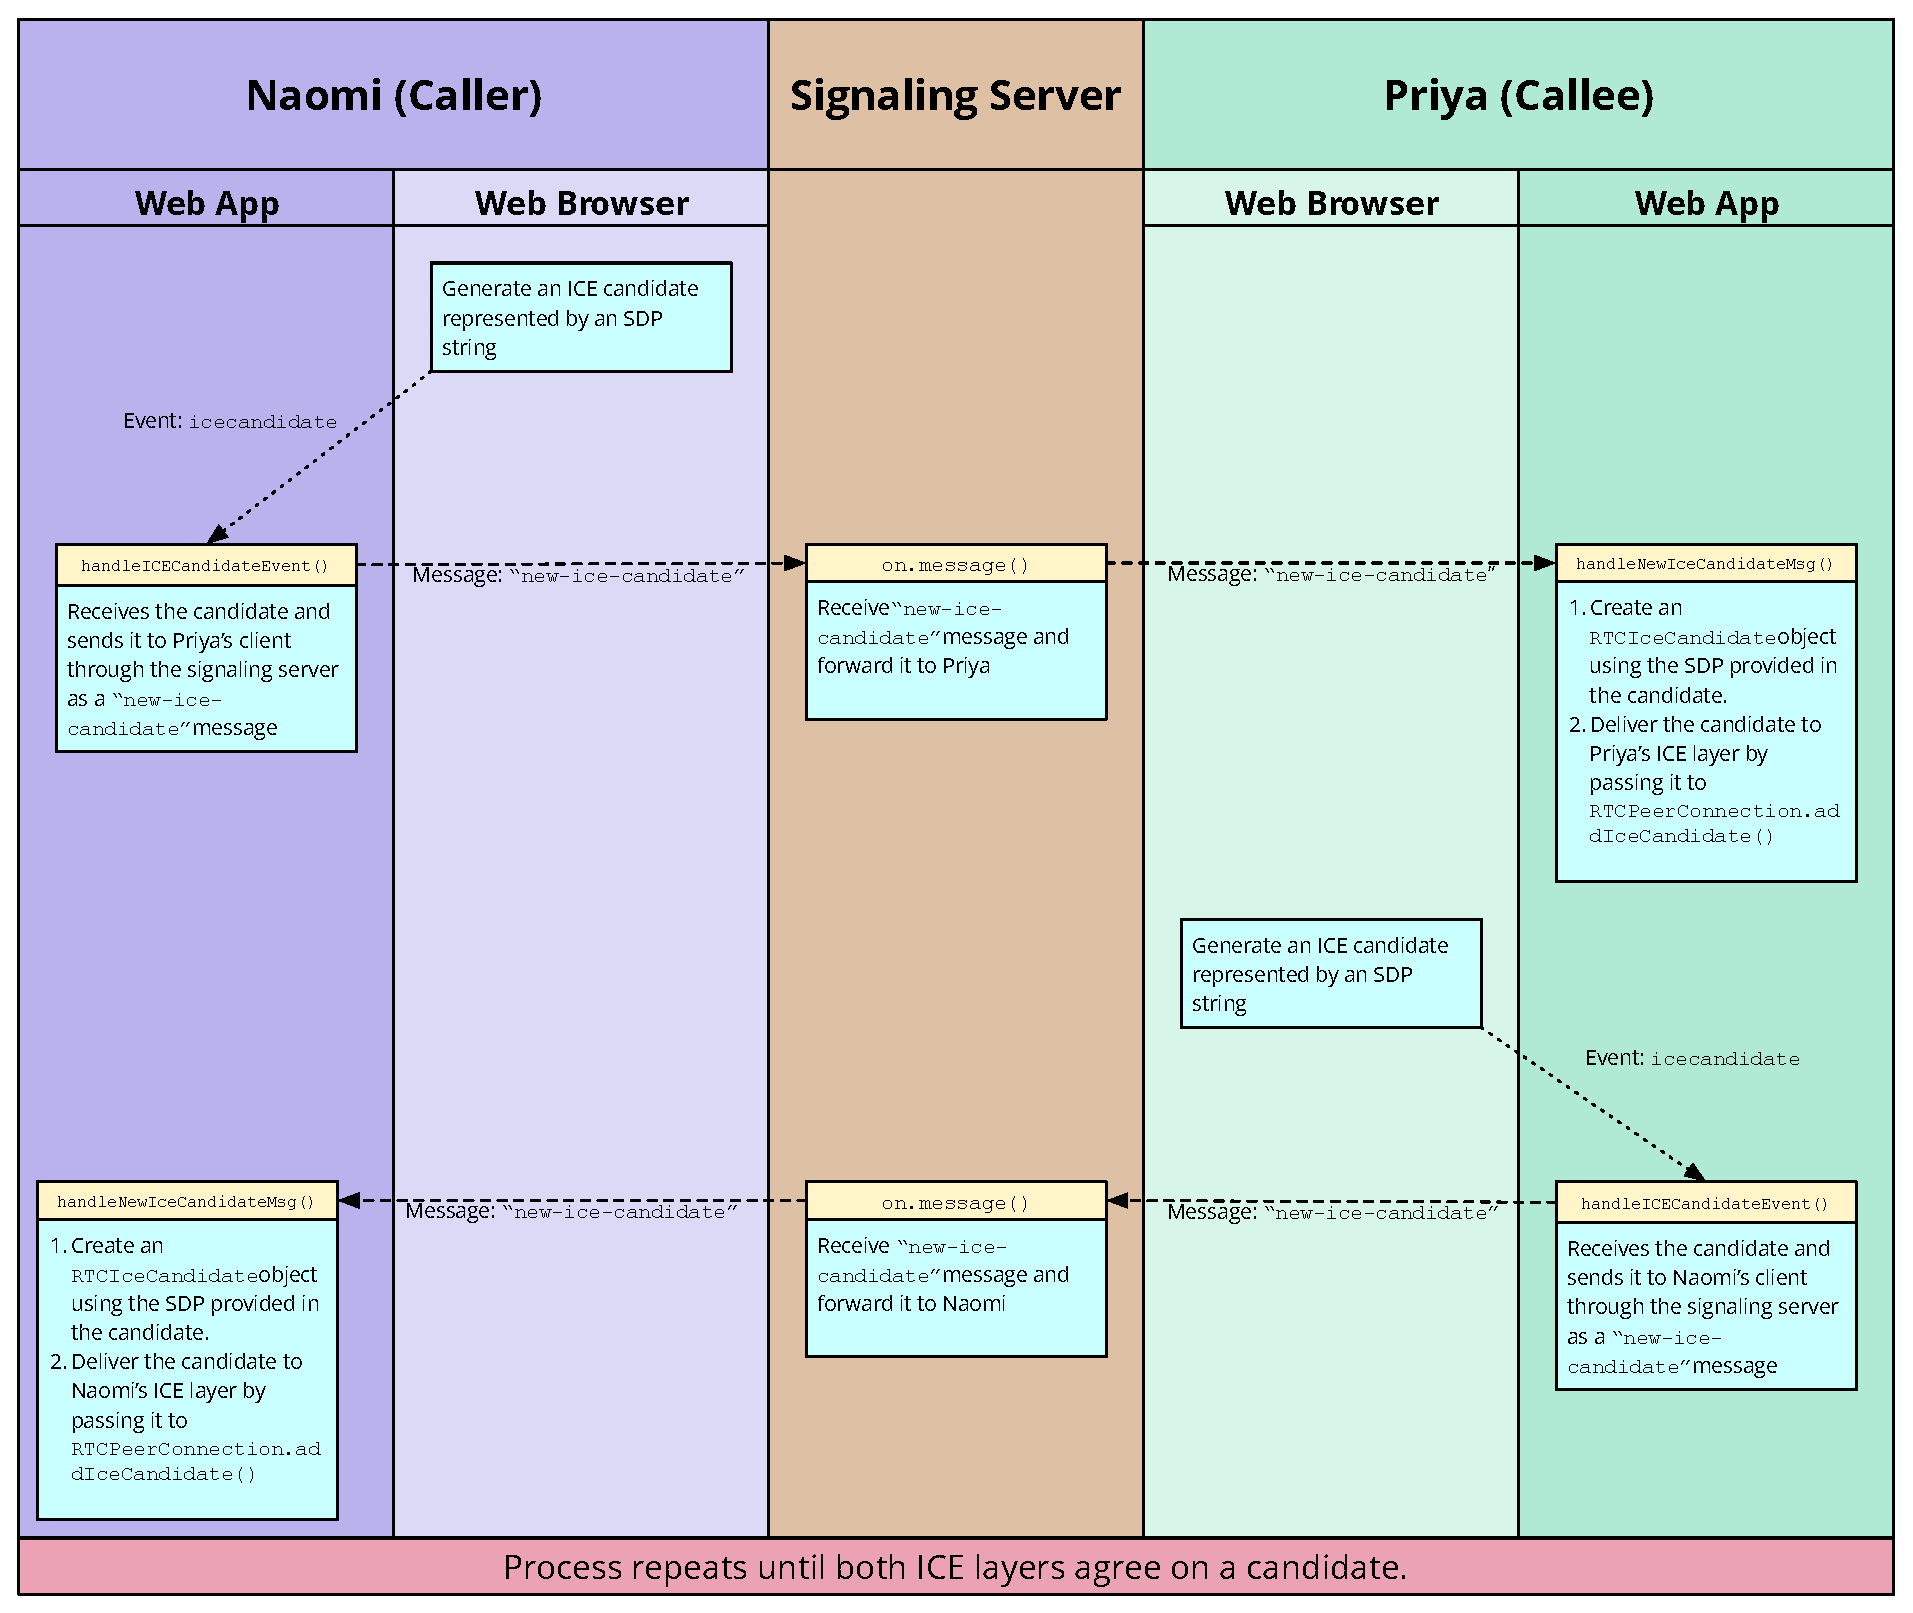
\includegraphics[width=1\textwidth]{images/ICECandidateExchange.pdf}
	\centering
	\caption{ICE communication schema, \url{https://mdn.mozillademos.org/files/12365/WebRTC - ICE Candidate Exchange.svg}}
	\label{fig:ICE Candidate Exchange}
\end{figure}

\lstinputlisting[label=ICE Candidates,caption=ICE Candidates,language=JavaScript, style=JavaScript]{examples/ICECandidate.js}